\documentclass[12pt, letterpaper]{article}
\usepackage{iarc_latex_style}
\usepackage{amssymb,amsmath,listings,url,verbatim,graphicx}

\title{BeoHawk: Autonomous Quadrotor}
\begin{document}
\maketitle
\begin{people}
\name{Christopher Li}
\org{University of Southern California}
\name{Rustom Jehangir}
\org{University of Southern California}
\end{people}

%1) Abstract	5
\begin{abstract}
	In this paper, we introduce a Micro UAV system that can explore an unknown indoor space without the assistance of a positioning system such as GPS. The robot takes in various kind of sensing measurements, handles them with probabilistic theories, and completes tasks such as stabilization and SLAM. \todo{Finish abstract at the end} (5 points)
\end{abstract}

%2) Introduction	5
%  a) Statement of the problem 
%  b) Conceptual solution to solve the problem
%    b1) Figure of overall system architecture 
%  c) Yearly Milestones
\section{Introduction (5)}
The USC Aerial Robotics Team's \textit{Beohawk} quadcopter was designed to suit the requirements of the International Aerial Robotics Competition. The quadcopter uses a variety of sensors to measure and identify the environment it is in with the effort of searching for small object in a complex and unknown setting.

\subsection{Problem Statement}
For the 6th IARC mission, our quadcopter must navigate an unknown office environment to find a small flash drive, retrieve it, and return in under ten minutes while avoiding detection.  The vehicle, which must weigh under 1.5kg, must operate autonomously, which introduces the challenge of mapping and navigating an environment sensed with instruments that have random errors and noise. 

\subsection{Conceptual Solution}
The USC Aerial Robotics Team is implementing a solution based on a traditional approach to robotics with modifications for the mission and for the mechanics of the robot. The quadcopter is custom built to be within the required weight and size range but uses a commercial control board for low level control. An onboard computer uses the Robotic Operating System (ROS) and takes advantage of many of the packages and tools made available by public contributors. 

\subsubsection{Figure of Overall System Architecture}

Figure \eqref{fig:architecture} shows the basic system architecture of the quadcopter. The quadcopter's low level control including stability, attitude control, altitude control, and position control are all performed by the low-level control board. This board is an Arduino based board that has sensors and motor outputs. It also receive radio-control signals and allows control to be over-ridden by a human pilot.

The main computer is a Pico-ITX form-factor x86 based computer that handles higher level control. This computer runs ROS, which performs optical flow calculations for basic positional stability. \sout{This computer also runs the navigator that decides where the robot will move and what actions it will take. More computationally expensive processes such as SLAM, take place on an off-board computer with a more powerful processor and more memory.} Mission planning, navigation, and SLAM take place on the base station, which has a more powerful processor and more memory. The quadcopter publishes sensor data and subscribes to navigation positions from the base station.

\begin{figure}[h]
\centering
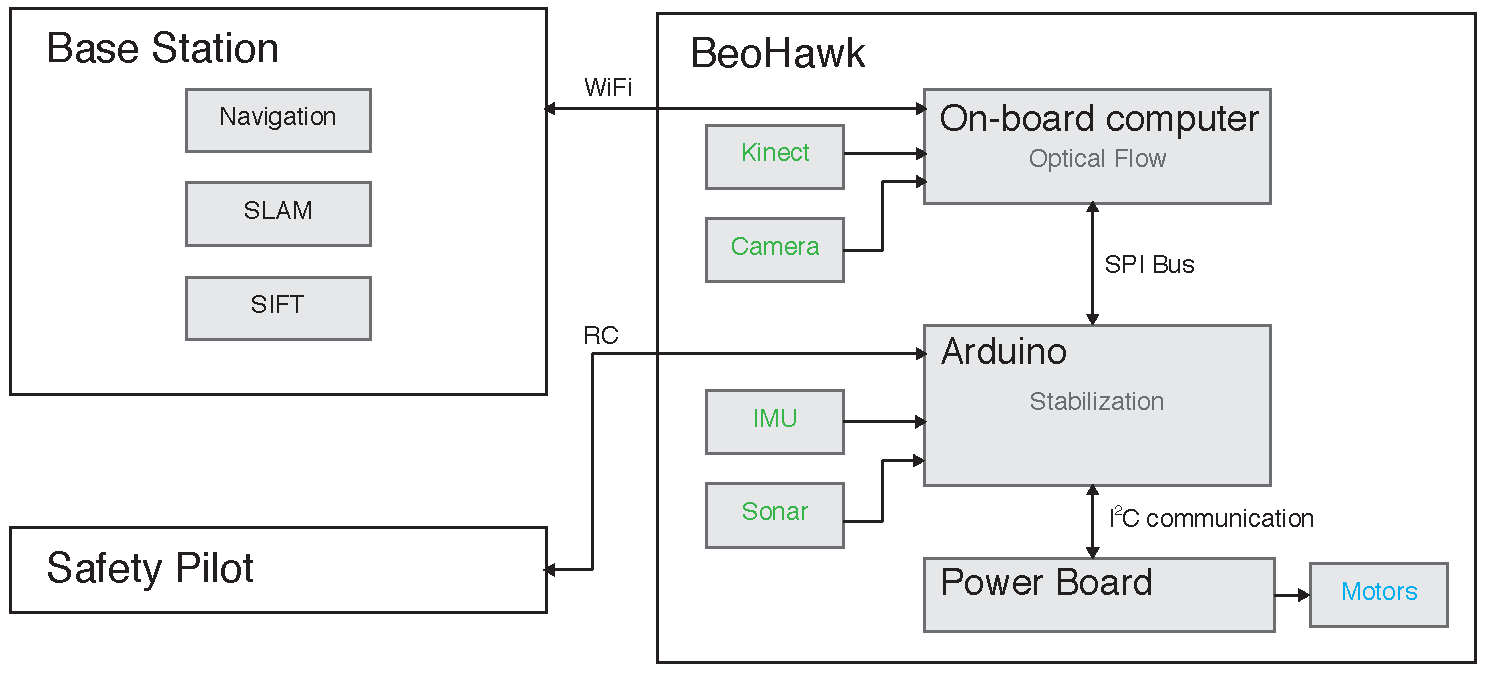
\includegraphics[width=14cm]{images/beohawk-system-arch.pdf}
\caption{General architecture of the Beohawk control system. \todo{This needs to be completed}.} 
\label{fig:architecture}
\end{figure}

\subsection{Yearly Milestones}
This is USC's first appearance at the IARC and our team's first competition. This year we hope to develop a platform capable of mapping and navigating the environment.  If we do not complete the goals, we will continue refining the quadcopter. \todo{eh.. feels lacking}

%3) Air Vehicle	15
%  a) Propulsion and Lift System 
%  b) Guidance, Nav., and Control 
%    b1) Stability Augmentation System 
%    b2) Navigation 
%    b3) Figure of control system architecture 
%  c) Flight Termination System
\section{Air Vehicle (15)}

\subsection{Propulsion and Lift System}
\emph{Beohawk} has four rotors, each an equal distance from the quadcopter's center.  Two opposite motors spin clockwise and the other two spin counter-clockwise, which generates a net torque of zero.  Hence, the quadcopter does not need a separate rotor to control yaw like a conventional helicopter, and can control yaw by adjusting the proportion of rotor speeds.  \todo{Todo: More details on these rotors}

\subsection{Guidance, Navigation, and Control}

\subsubsection{Stability Augmentation System}
\todo{Something about stability}

\begin{figure}[h]
\centering
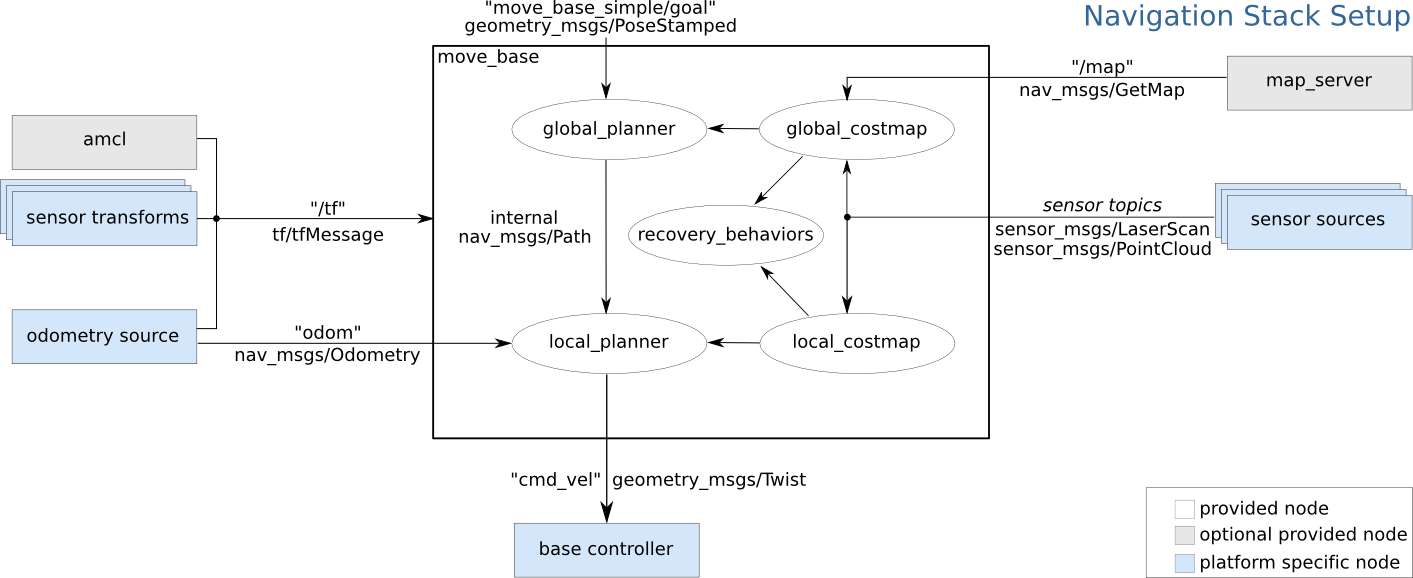
\includegraphics[width=12cm]{images/overview_tf.png}
\caption{Navigation system of Beohawk. \todo{This is a placeholder}.} 
\label{fig:navi}
\end{figure}

\subsubsection{Navigation}
Navigation is done in 2D using the navigation ROS package. Figure \eqref{fig:navi} shows the inputs to the navigation stack. Mission control is managed with a state machine that keeps track of the current objective.  \todo{Possibly a state diagram? To finish later}


\subsubsection{Figure of Control System Architecture}
All pages have 2.5cm (1 inch) margins on all sides. Only page numbers are allowed to violate margins. Papers are limited to 12 pages (including figures and references, if any). The format shall be single-sided with text occupying a space no greater than 22.86 cm (9 inches) tall by 16.51 cm (6.5 inches) wide centered on each page.

\subsection{Flight Termination System}
All pages have 2.5cm (1 inch) margins on all sides. Only page numbers are allowed to violate margins. Papers are limited to 12 pages (including figures and references, if any). The format shall be single-sided with text occupying a space no greater than 22.86 cm (9 inches) tall by 16.51 cm (6.5 inches) wide centered on each page.


%4) Payload	15
%  a) Sensor Suite 
%    a1) GNC Sensors 
%    a2) Mission Sensors 
%      a21) Target Identification 
%      a22) Threat Avoidance 
%  b) Communications 
%  c) Power Management System 
%  d) Sub-Vehicle (if any)
\section{Payload (15)}
\subsection{Sensor Suite}
\subsubsection{Microsoft Kinect}
The Kinect uses an infrared laser array of 640x480 points to provide depth information at 2048 levels of sensitivity. A ROS package uses the Kinect to produce a point cloud, which gives BeoHawk a plane of vision.

\subsubsection{Camera}
The quadcopter employs a downward facing camera to detect drift. The on-board computer runs an optical flow algorithm to reduce drift. \todo{Let's see that camera}

\subsubsection{Sonar}
The quadcopter also uses sonar to determine altitude. By fixing the altitude, BeoHawk can use 2D SLAM. \todo{More about sonar}

\subsubsection{Target Identification}
\todo{Reading signs}

\subsubsection{Threat Avoidance}
\todo{How will we dodge the laser tripwires?}

\subsection{Communications}
All pages have 2.5cm (1 inch) margins on all sides. Only page numbers are allowed to violate margins. Papers are limited to 12 pages (including figures and references, if any). The format shall be single-sided with text occupying a space no greater than 22.86 cm (9 inches) tall by 16.51 cm (6.5 inches) wide centered on each page.

\subsection{Power Management System}
All pages have 2.5cm (1 inch) margins on all sides. Only page numbers are allowed to violate margins. Papers are limited to 12 pages (including figures and references, if any). The format shall be single-sided with text occupying a space no greater than 22.86 cm (9 inches) tall by 16.51 cm (6.5 inches) wide centered on each page.

%5) Operations	10
%  a) Flight Preparations 
%    a1) Checklist(s) 
%  b) Man/Machine Interface
\section{Operations (10)}
All pages have 2.5cm (1 inch) margins on all sides. Only page numbers are allowed to violate margins. Papers are limited to 12 pages (including figures and references, if any). The format shall be single-sided with text occupying a space no greater than 22.86 cm (9 inches) tall by 16.51 cm (6.5 inches) wide centered on each page.

\subsection{Flight Preparations}
All pages have 2.5cm (1 inch) margins on all sides. Only page numbers are allowed to violate margins. Papers are limited to 12 pages (including figures and references, if any). The format shall be single-sided with text occupying a space no greater than 22.86 cm (9 inches) tall by 16.51 cm (6.5 inches) wide centered on each page.

\subsubsection{Checklists}
All pages have 2.5cm (1 inch) margins on all sides. Only page numbers are allowed to violate margins. Papers are limited to 12 pages (including figures and references, if any). The format shall be single-sided with text occupying a space no greater than 22.86 cm (9 inches) tall by 16.51 cm (6.5 inches) wide centered on each page.

\subsection{Man/Machine Interface}
The base station displays BeoHawk's current mission and status inferred from the sensor data returned by BeoHawk.  If the link is terminated, BeoHawk will attempt to hover in place until the connection is restored. In addition, the quadcopter will be connected to a human operator who will assume control of the quadcopter if anything goes wrong.


%6) Risk Reduction	15
%  a) Vehicle Status 
%    a1) Shock/Vibration Isolation 
%    a2) EMI/RFI Solutions 
%  b) Safety 
%  c) Modeling and Simulation 
%  d) Testing
\section{Risk Reduction}
\subsection{Vehicle Status}
BeoHawk transmits battery information, sensor information, and current objective to the base station. 

\subsubsection{Shock/Vibration Isolation}
\todo{Something about the material?}

\subsubsection{EMI/RFI Solutions}
Use tables and figures to concisely state your point. A table title appears above the table it references and appears in all caps and centered, whereas a figure title appears beneath the figure and with only leading capitalization. Both table and figure titles are italicized as shown in the examples below:

\subsection{Safety}
Use tables and figures to concisely state your point. A table title appears above the table it references and appears in all caps and centered, whereas a figure title appears beneath the figure and with only leading capitalization. Both table and figure titles are italicized as shown in the examples below:

\subsection{Modeling and Simulation}
Use tables and figures to concisely state your point. A table title appears above the table it references and appears in all caps and centered, whereas a figure title appears beneath the figure and with only leading capitalization. Both table and figure titles are italicized as shown in the examples below:

\subsection{Testing}
Use tables and figures to concisely state your point. A table title appears above the table it references and appears in all caps and centered, whereas a figure title appears beneath the figure and with only leading capitalization. Both table and figure titles are italicized as shown in the examples below:

\begin{table}[h]
\centering
\begin{tabular}{l  r  r  r}
                                       & Used  & Avail. & Perc. \\
  Number of Slices:                    &  684  & 4656  &  14\%  \\
  Number of Slice Flip Flops:          &  198  & 9312  &   2\%  \\
  Number of 4 input LUTs:              & 1316  & 9312  &  14\%  \\
  Number of IOs:                       &   37  &       &      \\
  Number of bonded IOBs:               &   36  &  232  &  15\%  \\
  Number of BRAMs:                     &    2  &   20  &  10\%  \\
  Number of MULT18X18SIOs:             &   10  &   20  &  50\%  \\
  Number of GCLKs:                     &    2  &   24  &   8\%  \\
\end{tabular}
\caption{Resource usage.}
\label{tab:usage}
\end{table}


%7) Conclusion	5 
\section{Conclusion (5)}
Use tables and figures to concisely state your point. A table title appears above the table it references and appears in all caps and centered, whereas a figure title appears beneath the figure and with only leading capitalization. Both table and figure titles are italicized as shown in the examples below:


%8) References	5
\bibliographystyle{IEEEbib}
\begin{thebibliography}{10}
\bibitem[1]{bib:kinectinfo} \url{http://git.marcansoft.com/?p=libfreenect.git;a=summary/}
\bibitem[2]{bib:mathworldfft} \url{http://mathworld.wolfram.com/FastFourierTransform.html}
\bibitem[3]{bib:ctdft} 	Cooley, J. W. and J. W. Tukey, ``An Algorithm for the Machine Computation of the Complex Fourier Series," Mathematics of Computation, Vol. 19, April 1965, pp. 297-301.
\bibitem[4]{bib:butterfly} Takala, J. and K. Punkka, ``Butterfly Unit Supporting Radix-4 and Radix-2 FFT," \url{http://ticsp.cs.tut.fi/images/4/48/Cr1028-riga.pdf}
\bibitem[5]{bib:fftdit} \url{http://cnx.org/content/m12016/latest/}
\bibitem[6]{bib:ffttricks} \url{http://cnx.org/content/m12021/latest/}
\end{thebibliography}


\end{document}